\documentclass[a4paper,11pt]{article}
\usepackage{amsmath,amssymb,latexsym}
\usepackage{cancel}
\usepackage[french]{babel}
\frenchbsetup{StandardLists=true} %important for bullet lists
\usepackage[T1]{fontenc}
\usepackage[utf8]{inputenc}
\usepackage{lmodern}
\usepackage{listings}
\usepackage[margin=2cm]{geometry}
\usepackage{microtype}
\usepackage{pdfpages}
\usepackage{hyperref}
\usepackage{graphicx}


\title{Seminar Public Service \\ Midterm Presentation}
\author{Maxime Piergiovanni \& Mathias Tonini}
\date{Autumn 2023}

\setlength\parindent{0pt}

\begin{document}

\maketitle

\section*{Problem : Difficulties in Implementing PER}

PER stands for "Plan d'Études Romand". It is a comprehensive plan for education and contains detailed  objectives for each learnings that students will undertake during their compulsory schooling \\

\url{https://portail.rpn.ch/administration/ens-or/Documents/Per_A3_Anglais_Web.pdf} \\

While Subject Areas (Languages, sciences, Arts...) take center stage and are well covered, including General Education and Cross Education in the Curriculum might provide more difficulties. \\

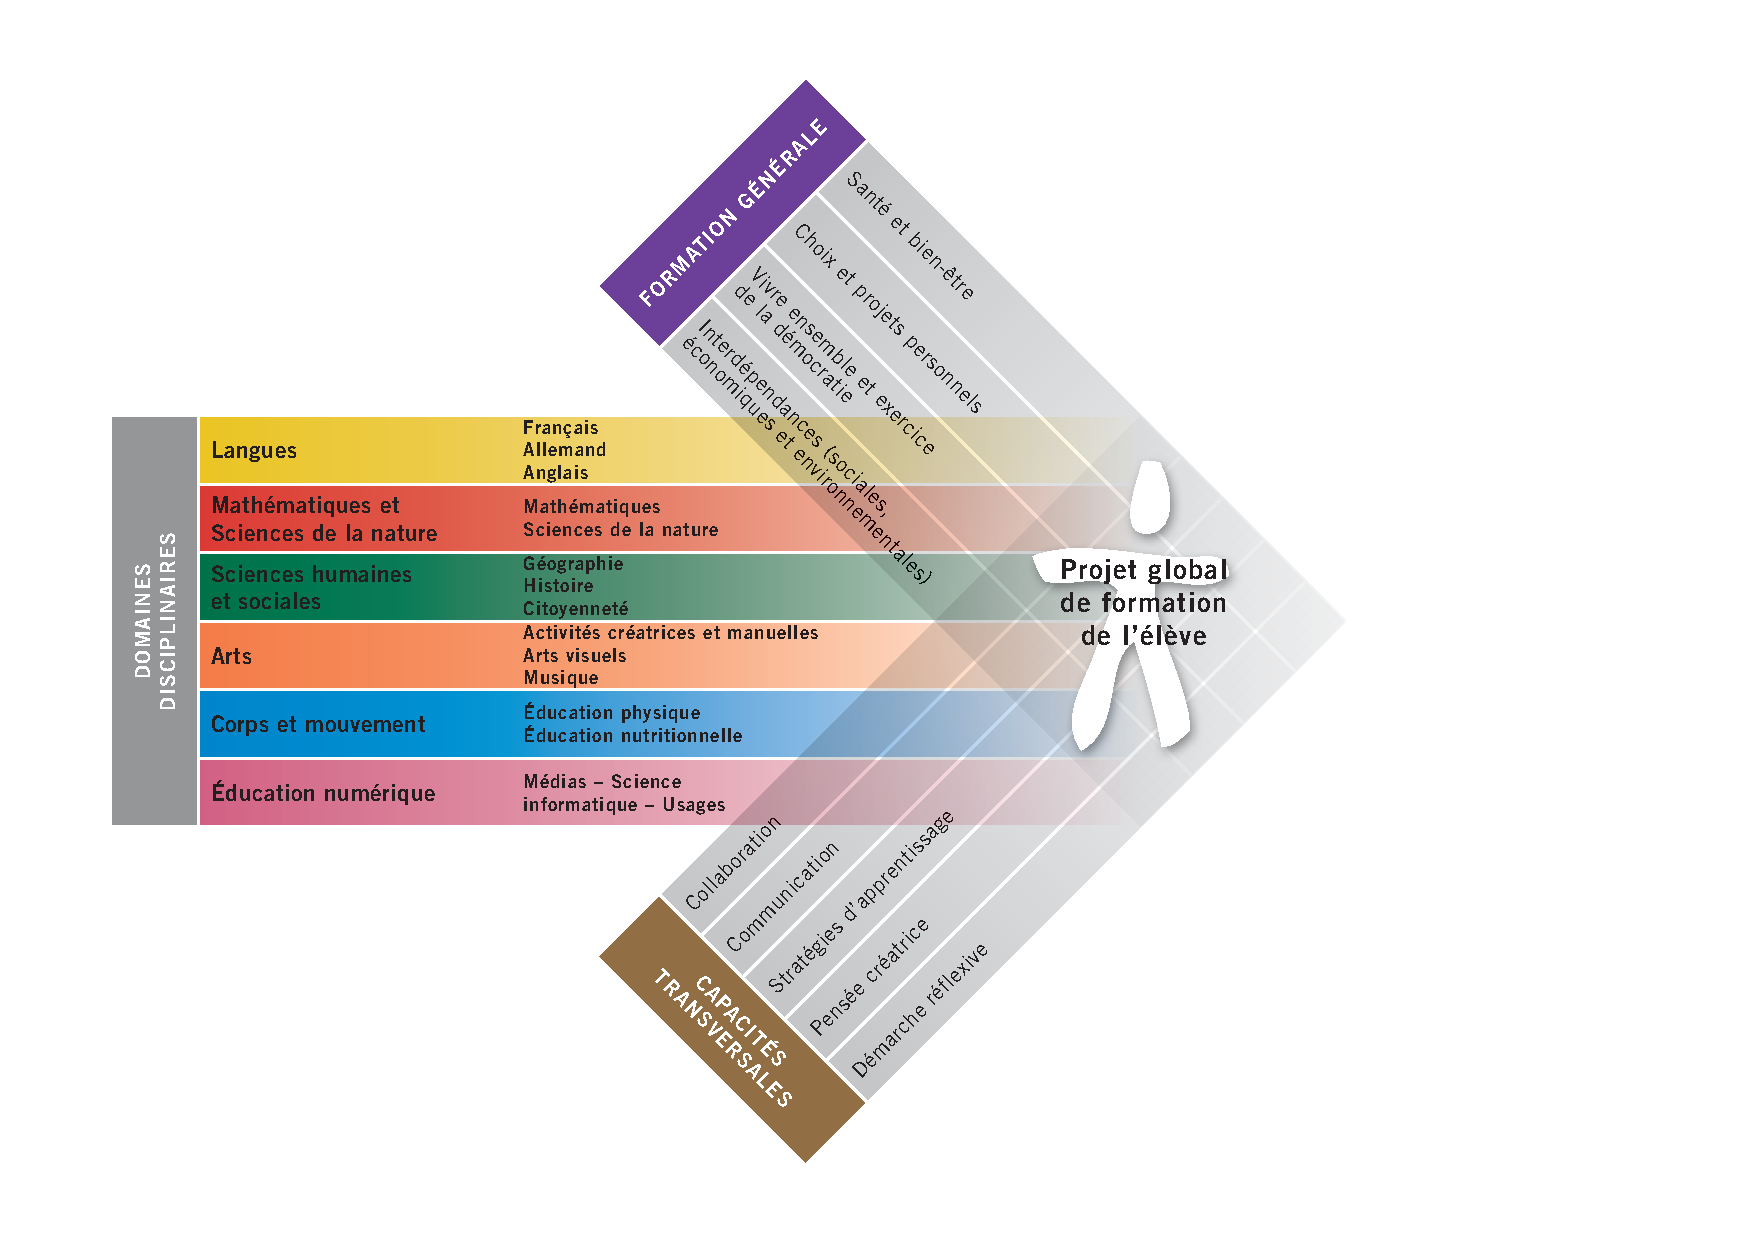
\includegraphics[scale=0.5]{./fleche_per.pdf}

The challenge grows when the number of teacher multiply, as is the case in cycle 3  (12 to 15 year olds). \\
The structure of the system is based on periods of time dedicated to a single subject and often given by a specific teacher. In this system, a teacher allowing time to a PER objective outside of its specific subject might fall behind in schedule. \\

\section*{State of the Art}

\url https://portail.ciip.ch/rn/resources \\

Our research yields that the platform in place allows for a simple and effective search of teaching units according to any PER objective. \\
Sharing teaching ressources doesn't seem to be the problem. \\


\section*{Artifact}

The proposed development focuses on communication between teachers. It introduces the concept of supra-sequences, that spans over a longer time period and across multiple subject. \\

The process would be initiated by one or more teacher and would give an overall goal to a given class. \\

Let's take an example for cycle 3 : FG 37 - Analyser quelques conséquences, ici et ailleurs, d'un système économique mondialisé (\url{https://portail.ciip.ch/per/learning-objectives/77}) \\
This over-arching goal opens up almost all individual subject to contribute to the supra-sequence. \\

Any teacher of the given class would be given access to the supra-sequence. The tool would show which teacher intend to give which unit. Any teacher is then free to join in the supra-sequence and plan a lesson accordingly.

Scheduling these supra-sequences woud need planning a long way ahead. The hope is to boost engagement with the non-subject PER objectives, and maybe in the process helping boost sharing of teaching units on the already existing tool.

\end{document}
